\chapter{Introduction to relevant topics}
\section{Graphene}
Graphene is a two-dimensional lattice of carbon atoms, arranged in a honeycomb structure as shown in the figure \ref{fig:graphene} Although it is straightforward to build many layers of these lattices (a substance known as graphite), it was long thought that a purely two-dimensional lattice would be unstable to thermal fluctuations and impossible to create.
This changed in 2004 when Andre Geim and Konstantin Novoselov succeeded in isolating two-dimensional graphene \cite{firstExfoliation}. For this, they won the 2010 Nobel prize. As we now show, the band structure of graphene is particularly interesting.
\begin{figure}[h]
    \makebox[\textwidth][c]{
        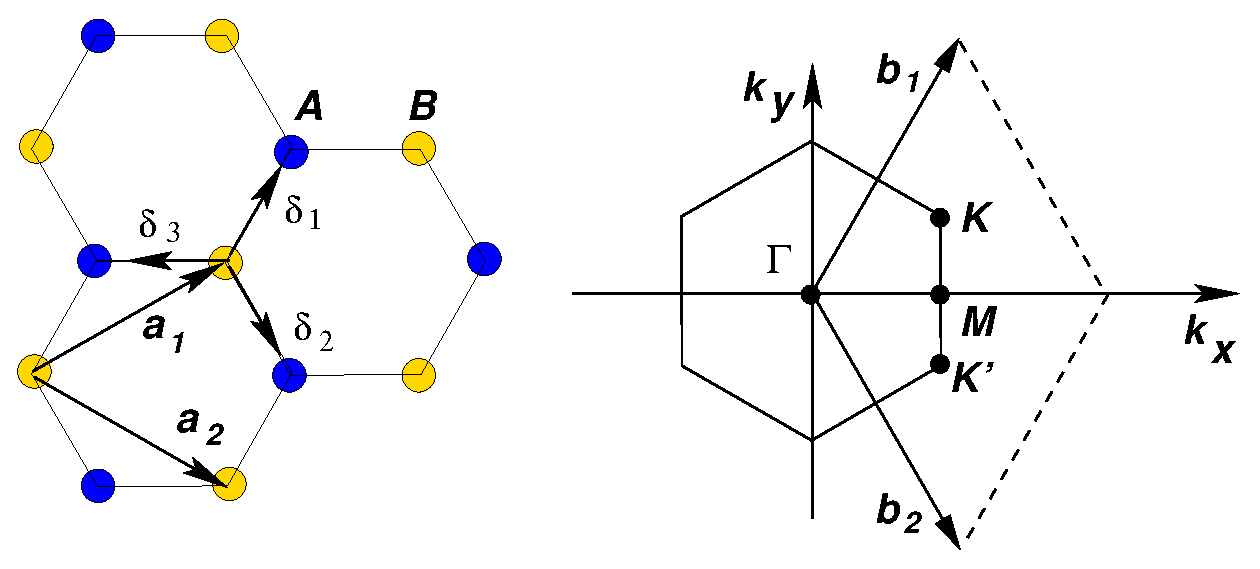
\includegraphics[width=\linewidth]{Immagini/graphene/structure.eps}
        }%
    \caption{On the left there is the lattice structure of graphene made out of two interpenetrating triangular lattices ($a_1$ and $a_2$ are the lattice unit vectors, and $\mathbf \delta_{i}$ with $i\in {1,2,3}$ are the nearest neighbors. On the right the corresponding Brillouin zone, the Dirac cones are located at the $K_0$ and $K_1$ points) \cite{guinea2008review}}
    \label{fig:graphene}
\end{figure}\\
We define the primitive lattice vectors $\vect a_1$ and $\vect a_2$ as follows:
\begin{equation}
    \vect a_1=\frac{a}2
    \begin{bmatrix}
        3 \\ \sqrt 3
    \end{bmatrix}\quad \quad
    \vect a_2=\frac{a}2
    \begin{bmatrix}
        3 \\ -\sqrt 3
    \end{bmatrix}
\end{equation}
Where $a$ is the distance between two neighboring atoms, which in graphene is $\approx 1.4\times 10^{-10}$m. The sublattice A is defined as all the points $\vect r = n_1\vect a_1 + n_2\vect a_2$ with $n_i \in \mathbb Z$ (yellow points in figure \ref{fig:graphene}), sublattice B is defined as all points $\vect r = n_1\vect a_1 + n_2\vect a_2 + \boldsymbol\delta$ with $\boldsymbol\delta = (a, 0)$ (blue points in figure \ref{fig:graphene}).

The reciprocal lattice vectors $\vect b_i$ are the vectors that satisfy $\vect a_i\cdot \vect b_j=\delta_{ij}$ and are equal to 
\begin{equation}
    \vect b_1=\frac{2\pi}{3a}\begin{bmatrix}
        1 \\ \sqrt 3
    \end{bmatrix}
    \quad \quad
    \vect b_2=\frac{2\pi}{3a}\begin{bmatrix}
        1 \\ -\sqrt 3
    \end{bmatrix}
\end{equation}
This reciprocal lattice is also triangular. The Brillouin zone is constructed in the usual manner by drawing perpendicular boundaries between the origin and each other point in the reciprocal lattice giving rise to a hexagonal Brillouin zone with $\vect K_0$ and $\vect K_1$ as the vertices of the hexagon, where 
\[
    \vect K_0=\frac 13 (2\vect b_1+\vect b_2)\quad \quad \vect K_1=\frac 13 (\vect b_1+2\vect b_2)
\]

\begin{equation}
   \vect K_0=\frac{2\pi}{3a}\left(1,\frac 1{\sqrt 3}\right)\quad\quad \vect K_1=\frac{2\pi}{3a}\left(1,-\frac 1{\sqrt 3}\right)
\end{equation}













\subsubsection*{The tight binding approach}
To investigate the band structure of graphene, we are going to use the tight binding approach \cite{bloch1929quantenmechanik,slater1954simplified}.
First we write the Hamiltonian.
\begin{equation}
    H=\frac{\vect p^2}{2m} + \sum_{\vect R\in C}V_a(x-\vect R)
    \label{eq:blochhamiltonian}
\end{equation}
Where $V_a$ is the potential of the single carbon atom, the set\\ $C=\left\{n_1\vect a_1 +n_2\vect a_2 + \nu\boldsymbol \delta\,|\,n_1,n_2\in \mathbb Z,\, \nu\in \{0,1\} \right\}$ is the set of all the positions of the atoms.\\ We can re-write the potential of the Hamiltonian in this more convenient manner.
\begin{equation}
    \sum_{\vect R\in C}V_a(x-\vect R) = V_a(x)+ V'(x)
\end{equation}
Where $V'(x)$ the potential of the other atoms, this way the can be divided in two parts:
\begin{equation}
    H=\underbrace{\frac{\vect p^2}{2m} + V_a(x)}_{\substack{\text{single-atom}\\\text{Hamiltonian}}} \,\,\,+ \underbrace{V'(x)}_\text{perturbation}
    \label{eq:blochhamiltoniandivided}
\end{equation}
Let $\ket{n,\vect R}$ be the $n$-th eingenstate of the Hamiltonian of single carbon atom placed in $\vect R$.
Due to translational symmetry, the wave function must satisfy the Bloch theorem, this tells us that the eingenstates of the Hamiltonian can be written as
\begin{equation}
    \ket{n,\nu,\vect k}=\sum_{\vect R_\nu\in C_\nu} e^{i\vect k \cdot \vect R_\nu}\ket{n,\vect R_\nu}
\end{equation}
with $\nu\in\{0,1\}$ and $C_\nu$ si defined as
\[
    C_\nu=\left\{n_1\vect a_1 +n_2\vect a_2 + \nu\boldsymbol \delta\,|\,n_1,n_2\in \mathbb Z\right\}
\]
With this we can now calculate the matrix elements of the Hamiltonian
\begin{equation}
    \big\langle n,\nu,\vect k\big|H\big| n',\nu',\vect k'\big\rangle=
    \sum_{\vect k\vect k',\vect R\vect R'}
    e^{i\vect k\cdot (\vect R +\nu\boldsymbol \delta)-i\vect k'\cdot(\vect R +\nu' \boldsymbol \delta)}
    \big\langle n,\nu,\vect R\big|H\ket{n',\nu',\vect R'}
\end{equation}
Since the matrix elements inside the summation don't depend on $k$ we have that the terms with $k\neq k'$ are equal to zero. So the equation above becomes
\[
    \big\langle n,\nu,\vect k\big|H\big| n',\nu',\vect k'\big\rangle= 
    \big\langle n,\nu,\vect k\big|H\big| n',\nu',\vect k\big\rangle\delta_{\vect k,\vect k'}
\]
This means that 
\[
    \big\langle n,\nu,\vect k\big|H\big| n',\nu',\vect k\big\rangle=
    \sum_{\vect k,\vect R\vect R'}
    e^{i\vect k\cdot (\vect R-\vect R' +\nu\boldsymbol \delta-\nu'\boldsymbol\delta)}
    \big\langle n,\nu,\vect R\big|H\ket{n',\nu',\vect R'}
\]
And, since it only depends on $\vect R-\vect R'$ we have that
\begin{equation}
    \label{eq:boh0}
    \big\langle n,\nu,\vect k\big|H\big| n',\nu',\vect k\big\rangle=
    \sum_{\vect k,\vect R}
    e^{i\vect k\cdot \vect R + i(\nu-\nu')\vect k\cdot \boldsymbol \delta}
    \big\langle n,\nu,\vect R\big|H\ket{n',\nu',\vect 0}
\end{equation}
Now we need to calculate the matrix elements $ \big\langle n,\nu,\vect R\big|H\ket{n',\nu',\vect 0}$. Using equation \ref{eq:blochhamiltoniandivided} we get that if $\vect R=\vect 0$
\begin{equation}
    \big\langle n,\nu,\vect 0\big|H\ket{n',\nu',\vect 0}
    =E_n\big\langle n,\nu,\vect 0\ket{n',\nu',\vect 0}+
    \big\langle n,\nu,\vect 0\big|V'(\vect r)\ket{n',\nu',\vect 0}
\end{equation}
For $\nu=\nu'$ the first term ($E_n\big\langle n,\nu,\vect 0\ket{n',\nu,\vect 0}=\delta_{nn'}$) and the second term, which is called crystal field integral is usually neglected because in most cases they simply produce a rigid shift of the energy bands $E_n(\vect k)$ without affecting their dispersion. \cite{grosso2013solid}\\
For $\nu\neq\nu'$ the second term is much bigger than the first one, so
\begin{equation}
    \big\langle n,\nu,\vect 0\big|H\ket{n',\nu',\vect 0}
    \approx E_n\delta_{nn'}\delta_{\nu\nu'}+
    \big\langle n,\nu,\vect 0\big|V'(\vect r)\ket{n',\nu',\vect 0}(1-\delta_{\nu\nu'})
    \label{eq:tight1}
\end{equation}
Since we consider the wavefunctions as strongly localized, the second term is much smaller than the first one, so we can ignore it.\\
Usually the matrix elements $\big\langle n,\nu,\vect 0\big|V'(\vect r)\ket{n',\nu',\vect 0}$ are conveniently expressed in terms of a a small number of independent parameters, and are evaluated either analytically, or numerically, or semi-empirically. 
\renewcommand{\arraystretch}{1.5}


In the case of carbon atoms we only need to work with atomic orbitals of type $s$ and $p$, this means that the independent matrix elements to evaluate are shown in table \ref{tab:matrix}
\begin{table}
    \label{tab:matrix}
    \begin{center}
        \begin{tabular}{l}
            \hline
            $\big\langle \,\,s\,,\nu,\vect 0\big|V'(\vect r)\ket{\,\,s\,,\nu',\vect 0}=V(ss\sigma)$\\
            $\big\langle \,\,s\,,\nu,\vect 0\big|V'(\vect r)\ket{p_x,\nu',\vect 0}=l_xV(sp\sigma)$\\
            $\big\langle p_x,\nu,\vect 0\big|V'(\vect r)\ket{p_x,\nu',\vect 0}=l_x^2V(pp\sigma)+(1-l_x^2)V(pp\pi)$\\
            $\big\langle p_x,\nu,\vect 0\big|V'(\vect r)\ket{p_y,\nu',\vect 0}=l_xl_y\left[V(pp\sigma)-V(pp\pi)\right]$\\
            $\big\langle p_x,\nu,\vect 0\big|V'(\vect r)\ket{p_z,\nu',\vect 0}=l_xl_z\left[V(pp\sigma)-V(pp\pi)\right]$\\
            \hline
        \end{tabular}
        \caption{ Here we have defined $\boldsymbol\delta=(l_x,l_y,l_z)|\delta|$}
    \end{center}
\end{table}

These parameters can be pictorially shown in figure \ref{fig:grapheneorbitals}
\begin{figure}[h]
    \makebox[\textwidth][c]{
        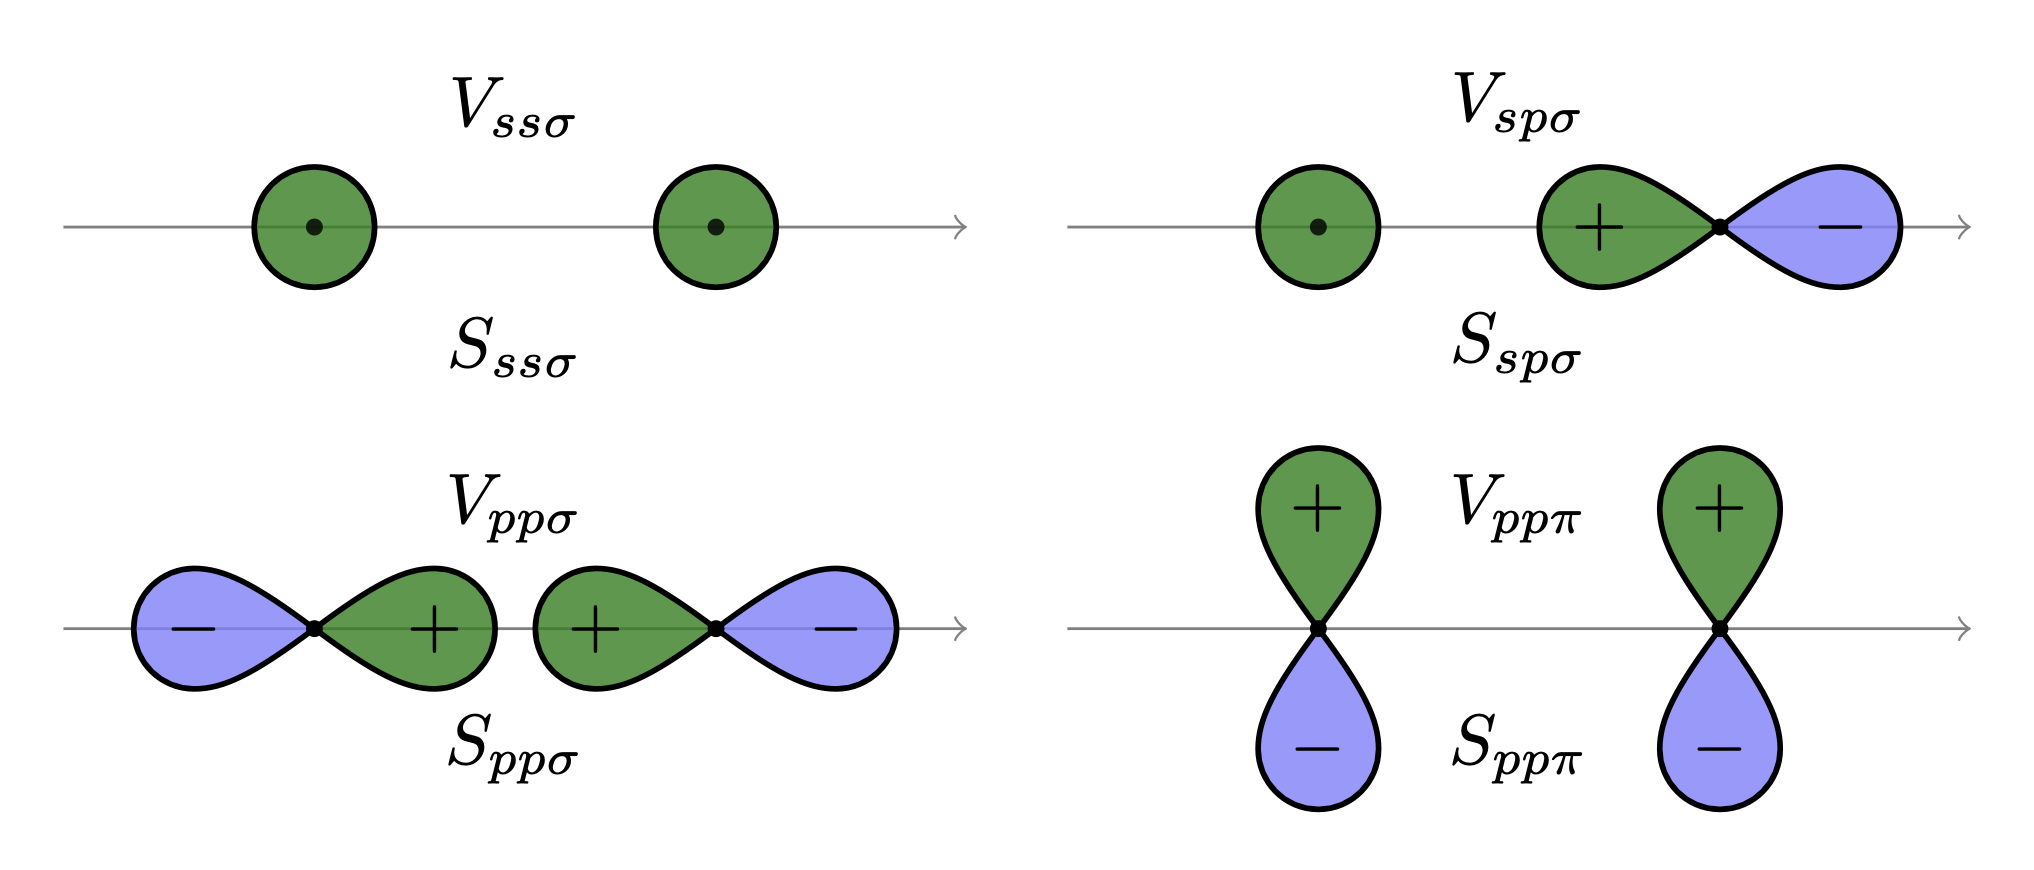
\includegraphics[width=\linewidth]{Immagini/graphene/orbitali_grafene.png}
        }%
    \caption{Each one of the potentials $V(ss\sigma),V(sp\sigma),V(pp\sigma),V(pp\pi)$ represent a different kind of bonding between the two orbitals. The first two indices represent the orbitals ($s$ and $p$), the last one represent the bonding type ($\sigma$ and $\pi$)}
    \label{fig:grapheneorbitals}
\end{figure}\\
The Hamiltonian matrix should be a $8 \times 8$ matrix. Nevertheless, from group theory we know that at a general point k the Bloch functions derived from $s$, $p_x$ and $p_y$ atomic functions never mix with the Bloch function $p_z$ because of the symmetry operation of reflection through the $xy$ plane. We can thus classify the energy states as even or odd with respect to this transformation; the former give rise to the so-called $\sigma$-bands and the latter to the so-called $\pi$-bands. Moreover, the problem is decomposed into two decoupled subproblems and, instead of diagonalizing a single $8 \times 8$ matrix, we have to cope separately with a $2 \times 2$ matrix ($\pi$-bands) and a $6 \times 6$ matrix
($\sigma$-bands).\\
Fortunately the $\sigma$-bands are fully below the Fermi-level, so they don't have any contribution to the electron-transport phenomenon, so we only have to deal with the $2\times 2$ matrix of the $\pi$-bands
\begin{equation}
    \big\langle p_z,\nu,\vect 0\big|H\ket{p_z,\nu',\vect 0}=
    \begin{bmatrix}
        E_p & V(pp\pi)\\
        V(pp\pi) & E_p
    \end{bmatrix}
\end{equation}

Now we can evaluate equation \ref{eq:boh0} considering just the nearest-neighbors
\begin{equation}
    \begin{split}
        \big\langle p_z,0,\vect k\big|H\ket{p_z,1,\vect k}=&
        \sum_{\vect k,\vect R}
        e^{i\vect k\cdot \vect R + i\vect k\cdot \boldsymbol \delta}
        \big\langle p_z,0,\vect R\big|H\ket{p_z,1,\vect 0}\approx\\
        \approx&\sum_{i}e^{i\vect k\cdot\vect \delta_i}
        V(pp\pi)\equiv\\
        \equiv&V(pp\pi)F(\vect k)
    \end{split}
\end{equation}


\begin{equation}
    \begin{split}
        \big\langle p_z,0,\vect k\big|H\ket{p_z,0,\vect k}=&
        \sum_{\vect k,\vect R}
        e^{i\vect k\cdot \vect R}
        \big\langle p_z,0,\vect R\big|H\ket{p_z,0,\vect 0}\approx E_p
    \end{split}
\end{equation}
Therefore, the $k$-dependent Hamiltonian for the $\pi$-bands is 
\begin{equation}
    \big\langle p_z,\nu,\vect k\big|H\ket{p_z,\nu',\vect k'}=\delta_{kk'}
    \begin{bmatrix}
        E_p & V(pp\pi)F(\vect k)\\
        V(pp\pi)F(\vect k) & E_p
    \end{bmatrix}
\end{equation}
